\documentclass[border=10pt]{standalone}

\usepackage{tikz}
\usepackage{tikzsymbols}
\usetikzlibrary{calc,patterns,shapes.geometric}

\def\centerarc[#1](#2)(#3:#4:#5){\draw[#1] ($(#2)+({#5*cos(#3)},{#5*sin(#3)})$) arc (#3:#4:#5);}

\begin{document}
	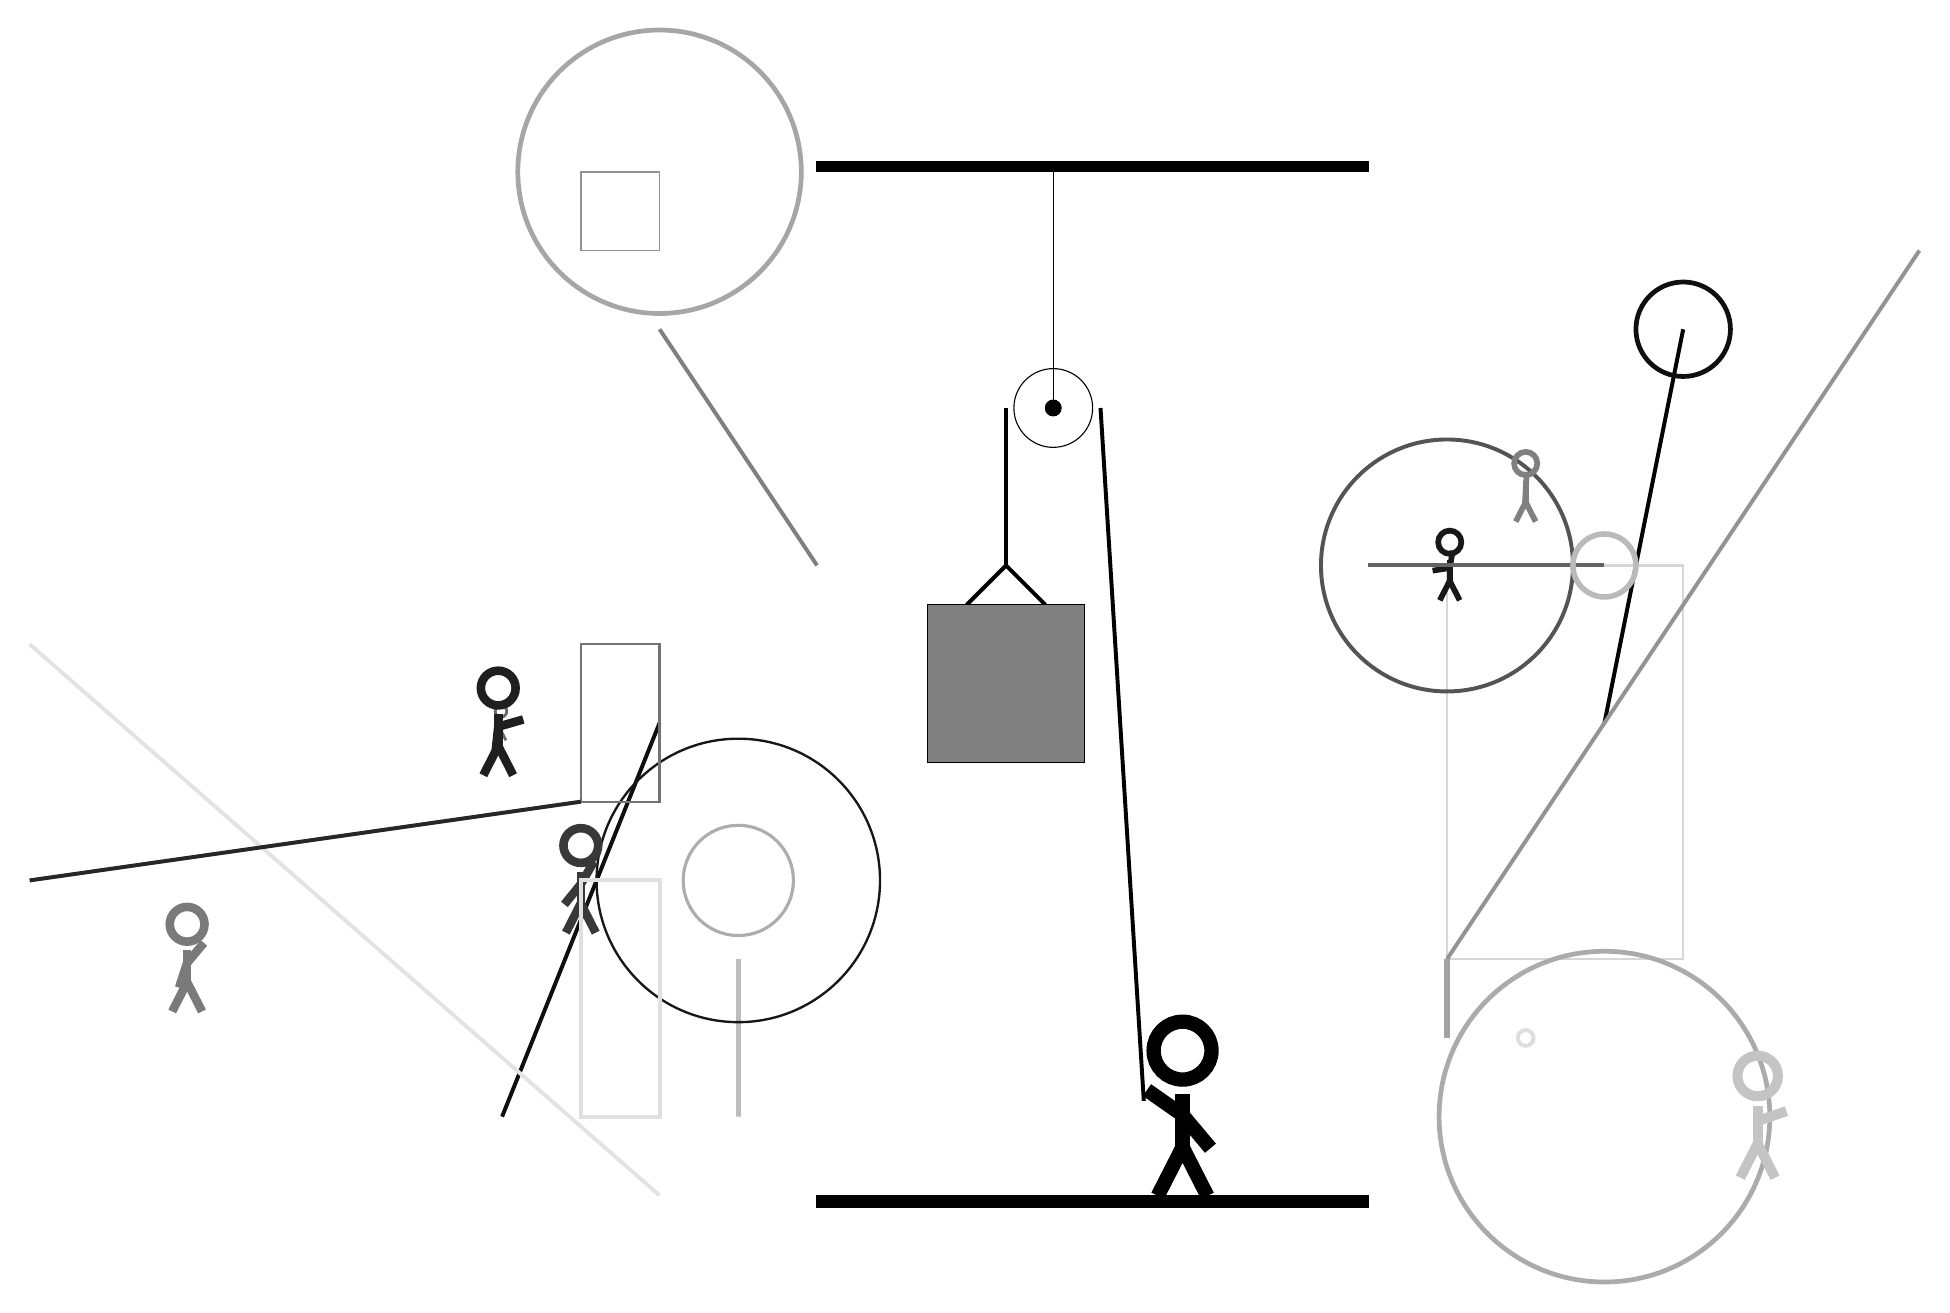
\begin{tikzpicture}
		%%%%% START %%%%%
		
		\draw[fill=black] (-2, 10) rectangle (5, 10.125);
		
		\draw (1, 7) circle (0.5);
		\draw[fill=black] (1, 7) circle (0.1);
		\draw (1, 10) -- (1, 7);
		
		\draw[line width=0.5mm] (-0.1, 4.5) -- (0.4, 5.0) -- (0.9, 4.5);
		\draw[fill=black!50] (-0.6, 4.5) rectangle (1.4, 2.5);
		
		\draw[line width=0.6mm, color=black!26] (-3, -2) rectangle (-3, 0);
		
		\draw[line width=0.3mm, color=black!16] (6, 5) rectangle (9, 0);
		\draw [line width=0.5mm, color=black!13](7, -1) circle (0.1);
		\draw[line width=0.5mm, color=black!94](-6, -2) -- (-4, 3);
		
		\draw[line width=0.5mm, color=black!99](8, 3) -- (9, 8);
		\draw[line width=0.5mm, color=black!42](6, 0) -- (12, 9);
		\draw [line width=0.3mm, color=black!91](-3, 1) circle (1.8);
		
		\draw[line width=0.5mm, color=black!11](-4, -3) -- (-12, 4);
		\draw [line width=0.6mm, color=black!35](-4, 10) circle (1.8);
		\draw [line width=0.5mm, color=black!67](6, 5) circle (1.6);
		\node[line width=0.7mm, color=black!90] at (6, 5) {\Strichmaxerl[4][9][80]};
		\node[line width=0.5mm, color=black!50] at (7, 6) {\Strichmaxerl[4][87][86]};
		\node[line width=0.2mm, color=black!78] at (-5, 1) {\Strichmaxerl[6][51][60]};
		
		\draw[line width=0.5mm, color=black!12] (-4, 1) rectangle (-5, -2);
		\draw[line width=0.2mm, color=black!43] (-4, 9) rectangle (-5, 10);
		\node[line width=0.6mm, color=black!52] at (-10, 0) {\Strichmaxerl[6][72][50]};
		\draw[line width=0.3mm, color=black!55] (-4, 2) rectangle (-5, 4);
		\draw[line width=0.7mm, color=black!36] (6, -1) rectangle (6, 0);
		\draw [line width=0.6mm, color=black!33](8, -2) circle (2.1);
		\node[line width=0.5mm, color=black!23] at (10, -2) {\Strichmaxerl[7][90][19]};
		\draw[line width=0.5mm, color=black!61](8, 5) -- (5, 5);
		
		\draw [line width=0.6mm, color=black!94](9, 8) circle (0.6);
		\node[line width=0.6mm, color=black!59] at (-6, 3) {\Strichmaxerl[2][83][23]};
		\draw [line width=0.4mm, color=black!32](-3, 1) circle (0.7);
		\node[line width=0.3mm, color=black!88] at (-6, 3) {\Strichmaxerl[6][84][16]};
		
		\draw[line width=0.5mm, color=black!85](-5, 2) -- (-12, 1);
		\draw [line width=0.7mm, color=black!27](8, 5) circle (0.4);
		\draw[line width=0.5mm, color=black!50](-4, 8) -- (-2, 5);
		
		\draw[line width=0.5mm] (0.4, 7) -- (0.4, 5.0);
		\centerarc[line width=0.5mm](1, 7)(0:180:0.6);
		\draw[line width=0.5mm](1.6, 7) -- (2.15, -1.8);
		
		\node at (2.6, -1.9) {\Strichmaxerl[10][-35][-50]};
		
		\draw[fill=black] (-2, -3) rectangle (5, -3.15);
		
		%%%%% END %%%%%
	\end{tikzpicture}
\end{document}